\documentclass[sigplan,screen]{acmart}

%% Contributed by Gregor von Laszewski
\usepackage{textcomp}
\usepackage{hyperref}
%\usepackage[table]{xcolor}

\usepackage{todonotes}
\newcommand{\TODO}[1]{\todo[inline]{#1}}
\newcommand{\NOTE}[1]{\textcolor{red}{[NOTE: #1]}}
\newcommand{\FILE}[1]{\todo[inline,color=green!20]{File: #1}}

\newcommand{\GITHUB}[1]{\todo[inline,color=green!20]{
\href{https://github.com/laszewsk/mlcommons-uva/issues/#1}{GitHub Issue #1}}}


\setcopyright{none}
\settopmatter{printacmref=false}
\renewcommand\footnotetextcopyrightpermission[1]{}

%\usepackage{minted}
%\setminted{fontsize=\footnotesize,xleftmargin=1.5\parindent}

\usepackage{longtable}
\usepackage{fancyvrb}

% \usepackage{color}
% \usepackage{listings}
%\usepackage{xcolor}
%\usemintedstyle{trac}
%\definecolor{mblue}{rgb}{0.27,0.33,0.53}

\definecolor{friendlybg}{HTML}{f0f0f0}
\definecolor{lightgray}{rgb}{.9,.9,.9}
\definecolor{darkgray}{rgb}{.4,.4,.4}
\definecolor{purple}{rgb}{0.65, 0.12, 0.82}

% \lstdefinelanguage{bash}{
%   keywords={cms, cd},
%   keywordstyle=\color{blue}\bfseries,
%   keywords=[2]{set},
%   keywordstyle=[2]\color{green}\bfseries,
%   identifierstyle=\color{black},
%   sensitive=false,
%   comment=[l]{//},
%   morecomment=[s]{/*}{*/},
%   commentstyle=\color{purple}\ttfamily,
%   stringstyle=\color{red}\ttfamily,
%   morestring=[b]',
%   morestring=[b]"
% }

% \lstset{
%   language=bash,
%   extendedchars=true,
%   basicstyle=\footnotesize\ttfamily,
%   showstringspaces=false,
%   showspaces=false,
%   tabsize=2,
%   breaklines=true,
%   showtabs=false
% }



%\setcopyright{acmcopyright}
%\copyrightyear{2018}
%\acmYear{2018}
%\acmDOI{XXXXXXX.XXXXXXX}

\acmConference[MLCommons Science Working Group Report]{MLCommons CloudMask Benchmark with Early Stopage }{Jun. 30,  revised 7 Dec. 2023}{Charlottesville, VA}

%\acmBooktitle{Woodstock '18: ACM Symposium on Neural Gaze Detection,
%  June 03--05, 2018, Woodstock, NY} 
%\acmPrice{15.00}
%\acmISBN{978-1-4503-XXXX-X/18/06}

%%\acmSubmissionID{123-A56-BU3}

%%\citestyle{acmauthoryear}

\begin{document}

\newcommand{\TITLE}{An Overview of MLCommons Cloud Mask Benchmark: \\ Related Research and Data \\ {\normalsize Version 1.0}}

\title[Overview of MLCommons Cloud Mask: Related Research]{\TITLE}
% \titlenote{\url{https://github.com/laszewski/papers/raw/master/vonLaszewski-cloudmask-related.pdf}, \url{https://arxiv.org/submit/5278659/view}}
\titlenote{\url{https://github.com/laszewski/papers/raw/master/vonLaszewski-cloudmask-related.pdf}}


\author{Gregor von Laszewski}
\email{laszewski@gmail.com}
\orcid{0000-0001-9558-179X}
\authornote{MLCommons authorized submitting author}
\affiliation{%
  \institution{University of Virginia}
  \streetaddress{Biocomplexity Institute and Initiative\\
Town Center Four\\
994 Research Park Boulevard}
  \city{Charlottesville}
  \state{VA}
  \postcode{22911}
  \country{USA}
}

\author{Ruochen Gu}
\email{bill.ruochen.gu@gmail.com}
\affiliation{%
  \institution{}
  \streetaddress{}
  \city{Shanghai}
  \state{}
  \postcode{}
  \country{CN}
}

\renewcommand{\shortauthors}{von Laszewski et al.}

\begin{abstract}

Cloud masking is a crucial task that is well-motivated for meteorology and its applications in environmental and atmospheric sciences. Its goal is, given satellite images, to accurately generate cloud masks that identify each pixel in image to contain either cloud or clear sky. 
In this paper, we summarize some of the ongoing research activities in cloud masking, with a focus on the research and benchmark currently conducted in MLCommons Science Working Group.
This overview is produced with the hope that others will have an easier time getting started and collaborate on the activities related to MLCommons Cloud Mask Benchmark.

\end{abstract}

\begin{CCSXML}
<ccs2012>
<concept>
<concept_id>10010405.10010432.10010437</concept_id>
<concept_desc>Applied computing~Earth and atmospheric sciences</concept_desc>
<concept_significance>500</concept_significance>
</concept>
<concept>
<concept_id>10010147.10010178.10010224.10010240.10010241</concept_id>
<concept_desc>Computing methodologies~Image representations</concept_desc>
<concept_significance>500</concept_significance>
</concept>
<concept>
<concept_id>10002951.10003317.10003359.10003360</concept_id>
<concept_desc>Information systems~Test collections</concept_desc>
<concept_significance>500</concept_significance>
</concept>
<concept>
<concept_id>10010583.10010737.10010749</concept_id>
<concept_desc>Hardware~Testing with distributed and parallel systems</concept_desc>
<concept_significance>500</concept_significance>
</concept>
</ccs2012>
\end{CCSXML}

\ccsdesc[500]{Applied computing~Earth and atmospheric sciences}
\ccsdesc[500]{Computing methodologies~Image representations}
\ccsdesc[500]{Information systems~Test collections}
\ccsdesc[500]{Hardware~Testing with distributed and parallel systems}



%%
%% Keywords. The author(s) should pick words that accurately describe
%% the work being presented. Separate the keywords with commas.
\keywords{cloudmask, cloudmesh, datasets, MLCommons, benchmark}


\received[Version from]{8. June, revised 7 December, 2023}

\begin{comment}
    
\begin{center}
{\huge\bf \TITLE}
\end{center}

% \listoftodos

\tableofcontents
\listoffigures
\listoftables

\clearpage
\end{comment}

\settopmatter{printfolios=true}
\maketitle


%%%%%%%%%%%%%%%%%%%%%%%%%%%%%%%%%%%%%%%%%%%%%%%%%%%%%
\section{MLCommons Cloud Mask Activities}
%%%%%%%%%%%%%%%%%%%%%%%%%%%%%%%%%%%%%%%%%%%%%%%%%%%%%

\nocite{las-2023-ai-workflow} % add to avoid running bibtex multiple times

The Cloud Mask Benchmark is part of the research currently conducted by MLCommons \cite{Farrell2021MLPerfHA} Science Working Group \cite{www-mlcommons-science-github}. 
We hope that others will contribute to this 
document to enhance its scope. Please contact Gregor von Laszewski (laszewski@gmail.com) 
so that we can coordinate with you.

As of this moment, we are aware of several activities regarding MLCommons Cloud Mask Benchmark.


\begin{enumerate}
\item The original benchmark was contributed by Samuel Jackson and Juri Papaya \cite{Thiyagalingam2022AIBF,jackson-2020-eu} from Rutherford Labs.
The reference implementation is based on U-Net \cite{RFB15a}. 

\item A cloud mask benchmark activity by Junji Yin on PEARL \cite{Thiyagalingam2022AIBF}.

\item A number of activities carried out by Gregor von Laszewski on Rivanna, University of Virginia's High Performance Computing Cluster. This activity contains significant contributions: 

    \begin{enumerate} 

    \item Introduction of a README to showcase how to run the code that has been reused and modified successfully by others.
      
    \item Introduction of target directories that showcase how to use templates to run cloudmask benchmarks on various HPC machines, DGX station, and a Linux desktop with an NVIDIA card.

    \item Introduction of enhanced timers to measure execution time for different parts of the benchmark program.

    \item Usage of Cloudmesh StopWatch to provide easy human readable timers that can be parsed with little effort through exports as CSV data.

    \item Development and usage of a hyper-parameter permutation framework that enables the cloud mask model to be experimented with different hyper-parameters, including epochs, batch sizes, learning rates, etc. This work is also reused in other MLCommons Science Benchmarks \cite{las22-cloudmesh-cc-reu}. The work simplies benchmark results following the FAIR principal while integrating the hyperparameters as metadata.

    \item Development of a workflow system that enables the use of hybrid compute resources through templates \cite{las-2023-escience-cloudmask}.

    \item Application of the aforementioned work to education \cite{las-2023-mlcommons-edu-eq}.

    \item Hosting of a development repository for MLCommons Cloud Mask Benchmark code base, as part of MLCommons Science Working Group \cite{github-laszewsk-mlcommons}.

    \item Execution of a substantial number of benchmark experiments.

\end{enumerate}

\item A number of activities by New York University ("NYU") AI for Scientific Research (AIFSR) Benchmark Team on Greene, NYU High Performance Computing Cluster. 

    \begin{enumerate}
        \item Modification of reference implementation to include early stoppage into model training, built onto the activities from Rutherford Labs and UVA.
        \item Implementation of a new accuracy metric introduced by Samuel Jackson, Juri Papaya, and Gregor von Laszewski.
        \item Coordinated the benchmark experiments with bash script that replicates a small number of features from the previous more comprehensive activity conducted by Gregor von Laszewski.
    \end{enumerate}

NYU AIFSR's benchmark activity contains a limited number of experiments in contrast to the activity done by Gregor von Laszewski. A joint report of both efforts is under preparation. Several versions of the report were started such as \cite{las23-cloudmask}. The latest report is not yet available.

\end{enumerate}


%%%%%%%%%%%%%%%%%%%%%%%%%%%%%%%%%%%%%%%%%%%%%%%%%%%%%
\section{Overview of Cloud Mask and its Related Work}
%%%%%%%%%%%%%%%%%%%%%%%%%%%%%%%%%%%%%%%%%%%%%%%%%%%%%

Since last century, several methods have been developed for cloud masking, ranging from rule-based techniques \cite{Saunders1986AnAS,Saunders1988AnIM,Merchant2005ProbabilisticPB, Zhu2012ObjectbasedCA} to modern deep learning approaches \cite{Li2019DeepLB,Domnich2021KappaMaskAC,Yan2018CloudAC,WIELAND2019111203,JEPPESEN2019247}. Among the more traditional, rule-based techniques, two popular methodologies have been threshold cloud screening \cite{Saunders1986AnAS,Saunders1988AnIM} and Bayesian cloud masking \cite{Merchant2005ProbabilisticPB}. 

Threshold screening methods consist of several threshold tests where spectral and spatial properties of satellite images are compared with those ranges that are believed to indicate the presence of a clear sky pixel. And those other pixels that are not labeled as clear sky are then flagged as cloudy. This school of methodologies were widely used from the late 1980s to the early 2000s \cite{Merchant2005ProbabilisticPB}. 

The gradual transition away from threshold screening methods was due to its long-criticized limitations: firstly, threshold settings rely heavily on domain expertise about indicators of cloudiness that may not be objective, which also makes later modification and updates difficult; secondly, thresholds provide users little flexibility in the trade-off between coverage and accuracy; third, threshold tests do not make use of all available prior information. These shortcomings of threshold screening methods are improved by later developed Bayesian methods \cite{Merchant2005ProbabilisticPB}.

The Bayesian approach applies Bayes' theorem on prior meteorology information to deduce for each pixel the probability of containing cloud or clear sky, and thereafter generating a cloud mask as output. As a result, these Bayesian approaches are fully probabilistic and make good use of prior information. Compared to threshold tests, Bayesian methods achieve better accuracy in predicting pixels' cloudiness, offering generality and conceptual clarity in its approach, and enhancing maintainability and adaptability largely \cite{Merchant2005ProbabilisticPB}. 

More recently, the rising popularity of deep learning has led to the use of CNNs for generating cloud masks. Deep learning methods \cite{Li2019DeepLB,Domnich2021KappaMaskAC,Yan2018CloudAC,WIELAND2019111203,JEPPESEN2019247} use computer vision models (CNNs) and treat the cloud mask task as that of image segmentation tasks. CNNs have achieved superior performance thanks to their automatic feature extraction ability. A research paper published in 2019 \cite{JEPPESEN2019247} introduces Remote Sensing Network (RS-Net), which is a CNN architecture branched out of U-Net \cite{RFB15a} for cloud masking and was shown to achieve higher performance compared to the state-of-the-art rule-based approach known as Fmask \cite{Zhu2012ObjectbasedCA}. KappaMask \cite{Domnich2021KappaMaskAC} and MSCFF \cite{Li2019DeepLB} are two additional U-Net based CNN model that outperformed Fmask. All these models have reported their performances on several satellite images such as Sentinel-2, Landsat, etc., and also made use of human-annotated (some assisted by software) ground truth values (See in Table \ref{tab:datasets}). On the other hand, MLCommons Cloud Mask Benchmark operates on SLSTR images from the newer Sentinel-3 satellite, which uses Bayesian approach generated cloud masks as ground truth. The reference implementation provided by MLCommons Science Working Group achieved 92\% classification accuracy on the Sentinel-3 test set \cite{Thiyagalingam2022AIBF}.

The aforementioned deep learning approaches towards cloud masking are by no means exhaustive. If you know about other significant cloud masking or deep learning approaches, please inform us and we will add them here. 

\begin{table*}[htb]
    \centering
    \caption{This table presents the several methods used for cloud masking with their respective dataset, ground truth, and performance.}
    \label{tab:datasets}
    \resizebox{1.8\columnwidth}{!}{
    \begin{tabular}{|l|c|l|l|l|l|}
    \hline
        {\bf} & {\bf Reference} & {\bf Dataset} & {\bf Ground-truth} & {\bf Model}  & {\bf Accuracy} \\ \hline
        1 & \cite{Merchant2005ProbabilisticPB} & ATSR-2 & Human annotation & Bayesian screening & 0.917\\ \hline
        2 & \cite{WIELAND2019111203} & Sentinel-2 & Software-assisted human annotation (QGIS) & U-Net & 0.90 \\ \hline
        3 & \cite{WIELAND2019111203} & Landsat TM & Software-assisted human annotation (QGIS) & U-Net & 0.89 \\ \hline
        4 & \cite{WIELAND2019111203} & Landsat ETM+ & Software-assisted human annotation (QGIS) & U-Net & 0.89 \\ \hline
        5 & \cite{WIELAND2019111203} & Landsat OLI & Software-assisted human annotation (QGIS) & U-Net & 0.91 \\ \hline
        6 & \cite{Li2019DeepLB} & GaoFen-1 & Human annotation & MFFSNet & 0.98, mIOU = 0.87 \\ \hline
        7 & \cite{Domnich2021KappaMaskAC} & Sentinel 2 & Software-assisted human annotation (CVAT) & KappaMask & 0.91 \\ \hline
        8 & \cite{JEPPESEN2019247} & Landsat 8 Biome and SPARCS & Human annotation & RS-Net & 0.956 \\ \hline
    \end{tabular}}

\end{table*}



%%%%%%%%%%%%%%%%%%%%%%%%%%%%%%%%%%%%%%%%%%%%%%%%%%%%%
\section{Dataset} 
%%%%%%%%%%%%%%%%%%%%%%%%%%%%%%%%%%%%%%%%%%%%%%%%%%%%%

For MLCommons Cloud Mask Benchmark, we use the satellite images from Sentinel-3. 

\subsection{Sentinel-3}

According to \cite{Sentinel84:online}
``Sentinel-3 is an ocean and land mission composed of two identical satellites (Sentinel-3A and Sentinel-3B).''

Sentinel-3 makes use of multiple sensing instruments to accomplish its objectives:

\begin{itemize}
    \item SLSTR (Sea and Land Surface Temperature Radiometer)
\item OLCI (Ocean and Land Colour Instrument)
\item SRAL (SAR Altimeter)
\item DORIS (Doppler Orbitography and Radiopositioning Integrated by Satellite)
\item MWR (Microwave Radiometer).

\end{itemize}

``SLSTR and OLCI are optical instruments that are used to provide data continuity for ENVISAT's AATSR and MERIS instruments and the swaths of the two instruments overlap, allowing for new combined applications. OLCI is a medium-resolution imaging spectrometer, using five cameras to provide a wide field of view.
SRAL, DORIS, MWR and LRR are used for topographic measurements of the ocean and inland water.'' \cite{Sentinel84:online}

One of the satellites is shown in Figure~\ref{fig:sat}. The 
Mission Orbit is 
sun-synchronous, set at a height of  814.5km
with an inclination of 98.65$^{o}$ and a repeat cycle of 27 days \cite{Sentinel84:online}.


\begin{figure}[htb]
\centering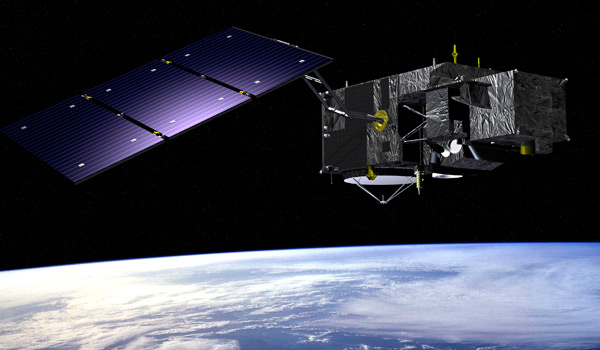
\includegraphics[width=0.8\columnwidth]{images/sentinel-3.jpg}
\caption{A Sentinel-3 Satelite.}
\label{fig:sat}
\end{figure}

\subsection{MLCommons Cloud Mask Dataset}

MLCommons Cloud Mask Benchmark uses 180GB of satellite images from Sentinel-3 SLSTR (Level-1 processing, TOA Radiances and Brightness Temperature) satellite images. The dataset consists of 1070 images, captured during days and nights. The dataset also includes a cloud mask for each image, generated using Bayesian techniques. The reference implementation uses these cloud masks as ground truths for training and testing.

The dataset comes with the train-test split, where 970 images are used for training, and 100 images are used for testing. 
The images are of the dimension $1200 \times 1500$ with 15 different channels and 1 channel of Bayesian mask. Among the 15 channels, 3 channels are used to represent brightness, 6 channels are used to represent reflectance, and the remaining 6 channels are used to represent radiance. However, for the provided reference implementation, only a total of 10 channels, i.e., 6 channels of reflectance, 3 channels of brightness, and 1 channel of Bayesian mask are used as model inputs for training and testing. 

\begin{figure*}[htb]

\centering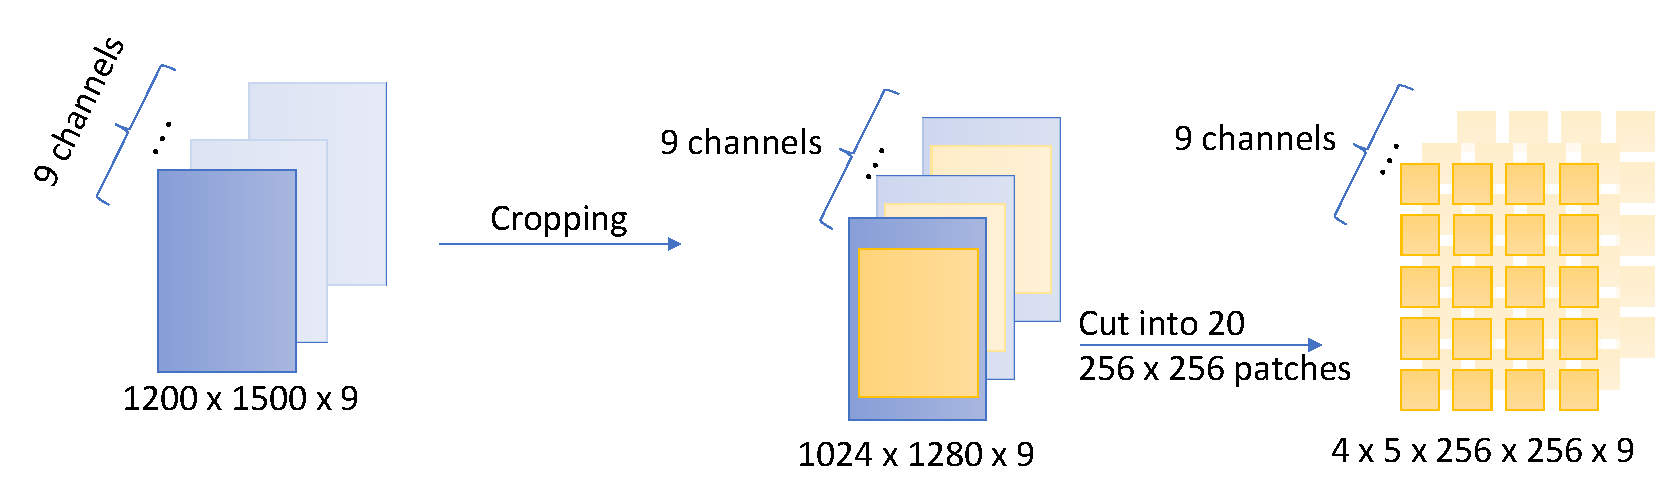
\includegraphics[width=0.75\textwidth]{images/cloudmask-preprocessing-training-data-2.pdf}
\caption{The preprocessing of the training data.}
\label{fig:preprocessing-training}

\bigskip

\centering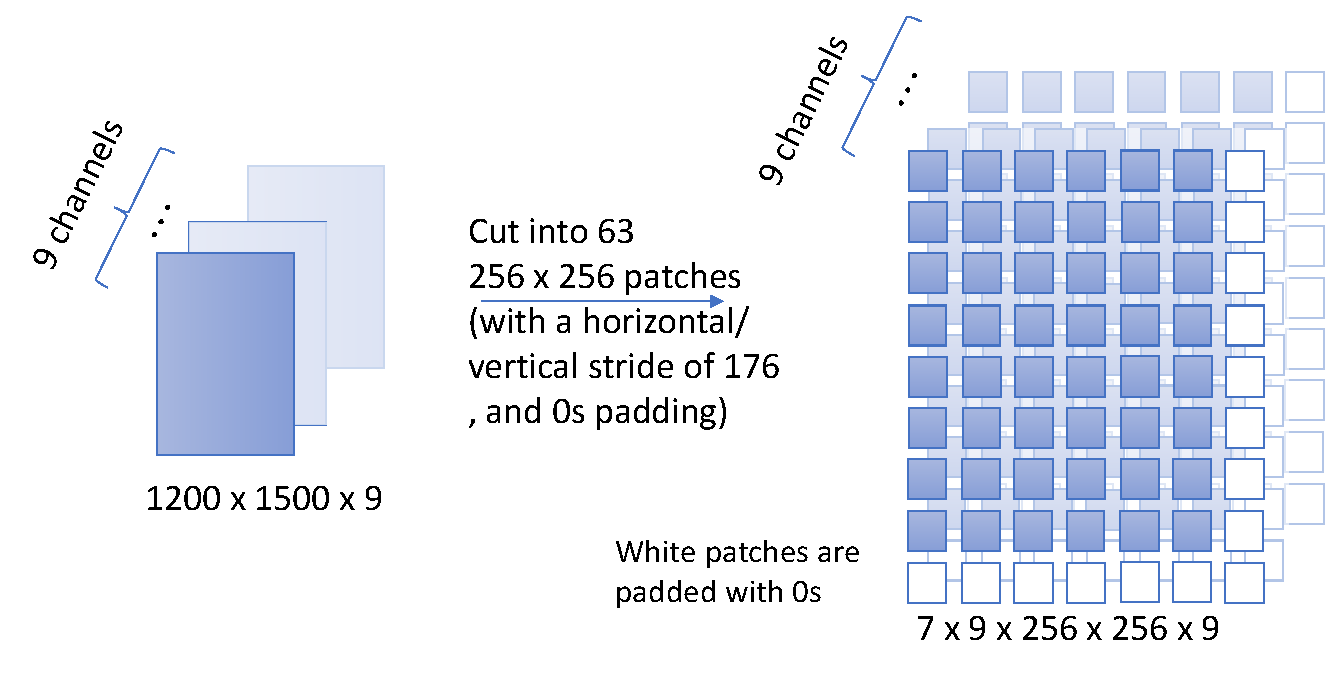
\includegraphics[width=0.75\textwidth]{images/cloudmask-preprocessing-testing-data-2.pdf}
\caption{The preprocessing of testing data}
\label{fig:preprocessing-testing}

\end{figure*}


\subsection{Data Loading and Preprocessing} \label{Preprocessing}

For training data preprocessing, the images are first cropped from the dimension of $1200 \times 1500 \times 9$ to $1024 \times 1280 \times 9$ and then divided into 20 smaller-sized $256 \times 256 \times 9$ patches. After creating these patches out of each image in training set, we get a total of $19400$ patches for training. These patches are further split into training and validation set with $80/20$ split ratio, and then sent for training after shuffling. 

For the test dataset, the images are neither cropped nor shuffled. Instead, each test image are cut into 63 smaller patches of dimension $256 \times 256 \times 9$, by applying a horizontal and vertical stride of 176 pixels with zeros padding on the right and bottom edges of each image. We then get a total of $6300$ patches for entire test dataset. After getting the predictions from the model, these $256 \times 256 \times 1$ output patches (predicted cloud mask) are reconstructed to the size of $1200 \times 1500 \times 1$ and then evaluated with the Bayesian mask ground truth that has the same dimension. This preprocessing pipelines for training and testing are shown in Figure \ref{fig:preprocessing-training} and Figure \ref{fig:preprocessing-testing}.

\subsection{Training}

During training, the model takes a preprocessed patch of dimension $256 \times 256 \times 9$, and generates a cloud mask of dimension $256 \times 256 \times 1$. Once the cloud masks have been generated by the model during training, the accuracy is reported as the percentage of total pixels that are correctly classified compared to ground truth. 

\subsection{Testing}

During testing, the model generates a cloud mask of dimension $256 \times 256 \times 1$ for each $256 \times 256 \times 9$ patch. For each pixel in the image, the model outputs the probability of that pixel containing clear sky. Pixels that have a probability higher than 50\% are labeled as clear sky, and cloudy otherwise. Then, those patches are then reconstructed back to full-size masks of dimension $1200 \times 1500 \times 1$. 

The locations of the images used in the testing are depicted in Figure~\ref{fig:frames-inference} as well as their coordinate centers in Figure~\ref{fig:frames-dot}. As one can observe from the figures, most of the testing images are captured in the region of North Altantic Ocean and of the West Coast of Europe.
Furthermore, we display in Figure \ref{fig:frames-raw} the raw satellite images from the Sentinel-3 database that reflect the locations where the testing images are located. Figure \ref{fig:frames-mask} shows the cloud masks of the testing images.
The Table \ref{tab:inference} shows the individual attributes for the specific locations identified by a counter.

\begin{figure*}[htb]
\centering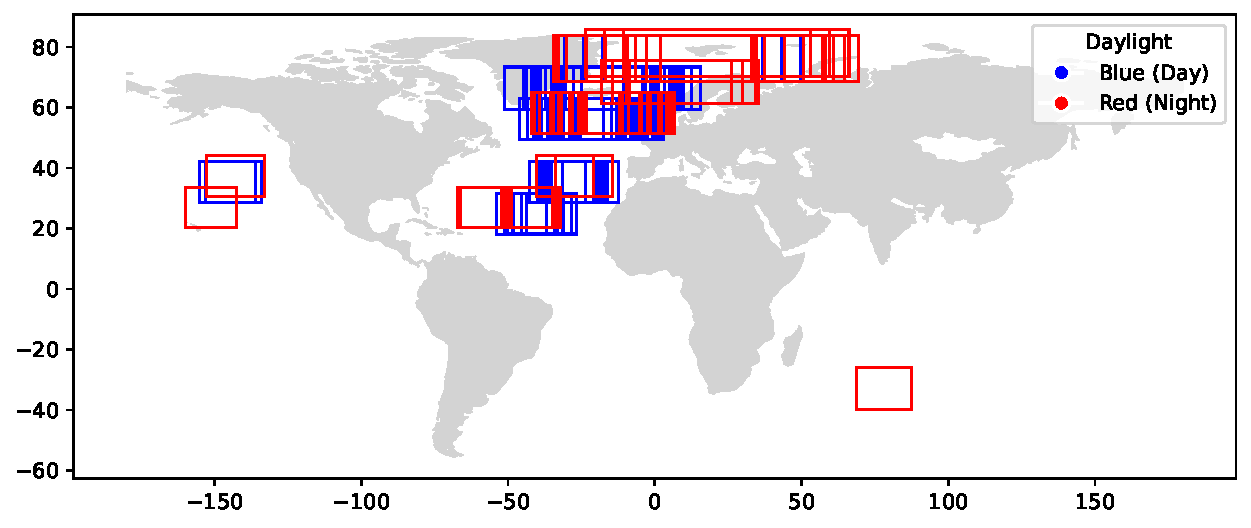
\includegraphics[width=0.75\textwidth]{images/inference-frames.pdf}
\caption{The location of the satellite images represented as frames used for inference.}
\label{fig:frames-inference}

\centering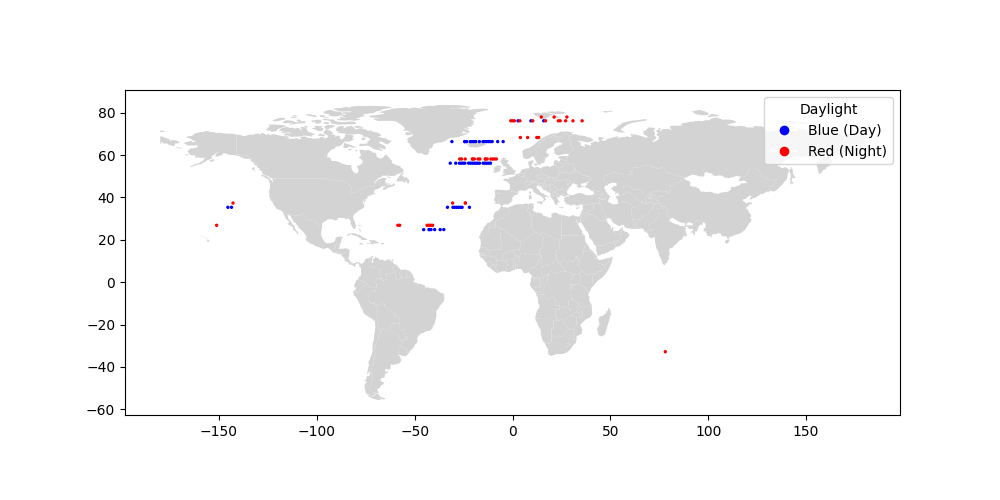
\includegraphics[width=0.8\textwidth]{images/inference-dots.png}
\caption{The location of the center of the satellite images used for inference.}
\label{fig:frames-dot}
\end{figure*}

\begin{figure*}[htb]
\centering\includegraphics[width=0.8\textwidth]{images/raw-output.png}
\caption{The raw satellite images at the locations where inference is chosen.}
\label{fig:frames-raw}
\end{figure*}

\begin{figure*}[htb]
\centering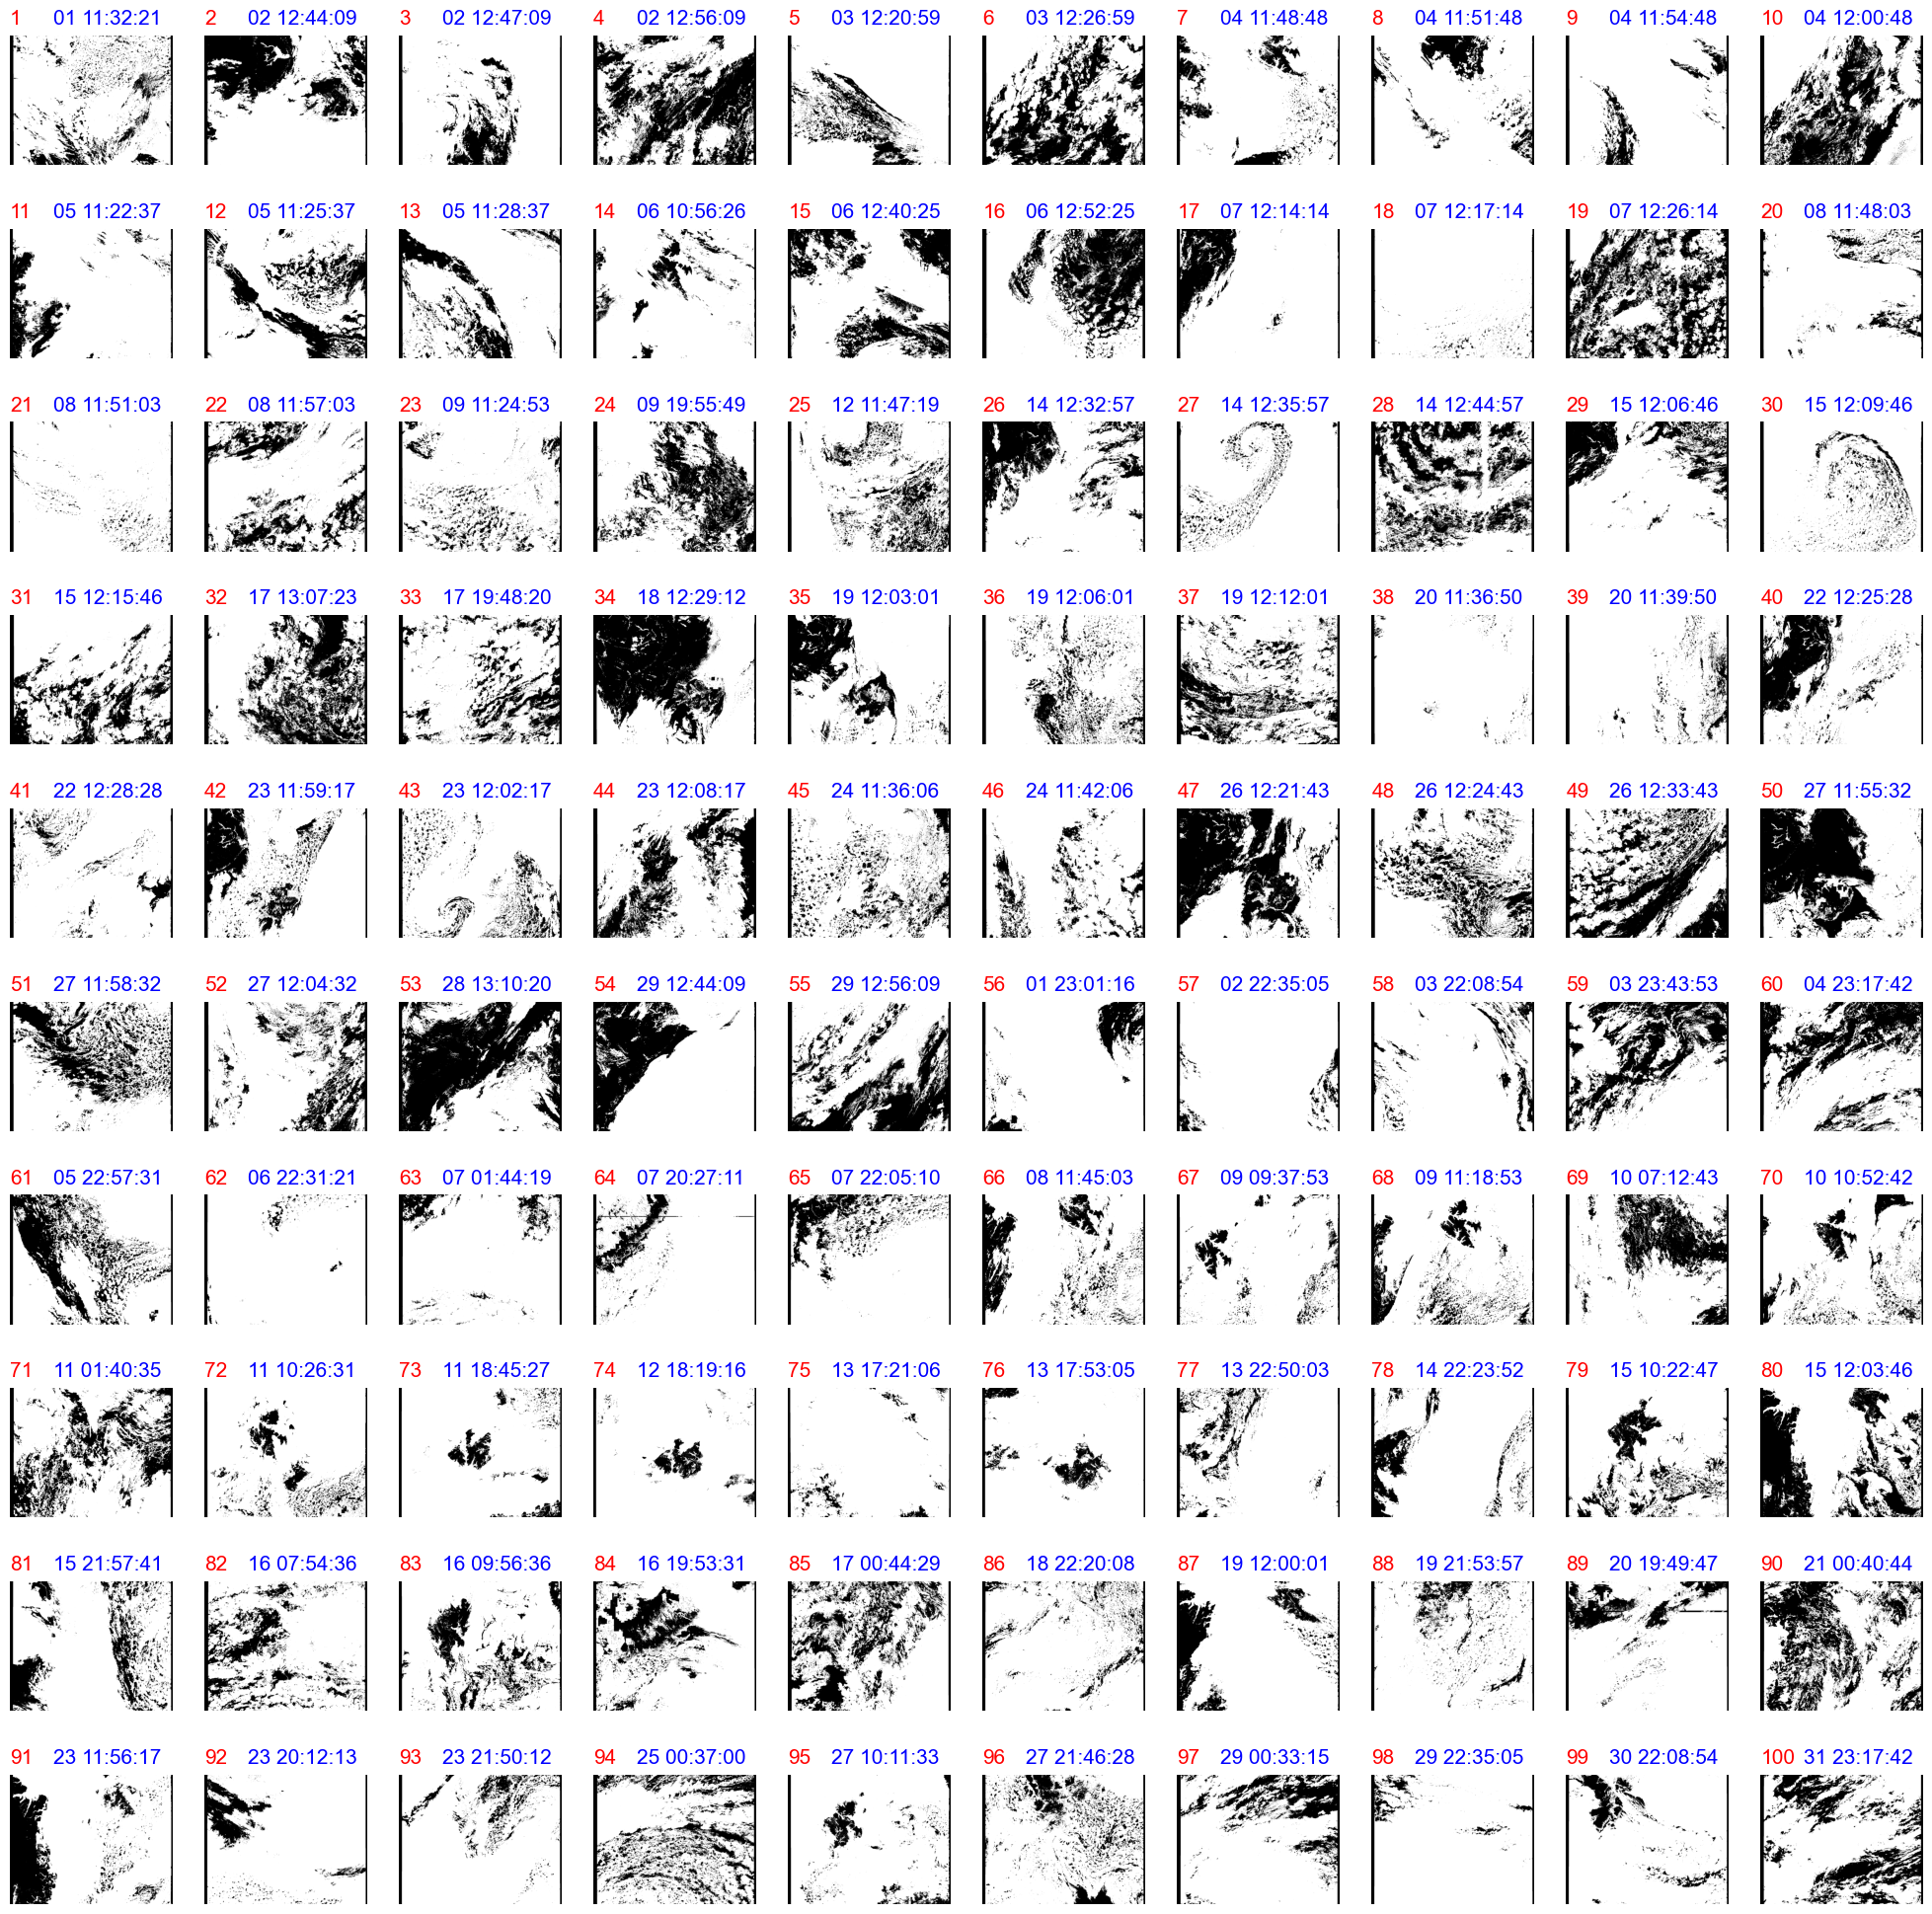
\includegraphics[width=0.8\textwidth]{images/masks-output.png}
\caption{The mask images at the locations where inference is chosen.}
\label{fig:frames-mask}
\end{figure*}



%%%%%%%%%%%%%%%%%%%%%%%%%%%%%%%%%%%%%%%%%%%%%%%%%%%%%
\section{Conclusion}
%%%%%%%%%%%%%%%%%%%%%%%%%%%%%%%%%%%%%%%%%%%%%%%%%%%%%


In this paper, we provide a list of related activities under MLCommons Cloud Mask Benchmark. The paper includes an overview of related research in the field of cloud masking in general. In addition, the paper provides a walk-through and illustration of the Sentinel-3 satellite image dataset used for MLCommons Cloud Mask Benchmark. With this paper, we hope to enhance communication between activities on this benchmark and support others to have an easier time getting started with the MLCommons Cloud Mask benchmark.

\begin{acks}

Work was in part funded by (a) NIST 60NANB21D151T  (b) NSF CyberTraining: CIC: CyberTraining for Students and Technologies from Generation Z with the award numbers 1829704 and 2200409 and NIST 60NANB21D151T, and (c) Department of Energy under the grant Award No. DE-SC0023452. The work from the UVA team was conducted at the Biocomplexity Institute and Initiative at the University of Virginia.
We like to thank the NYU AIFSR team for their contributions. We especially like to thank Ruochen Gu who continued to work on this project on voluntary basis.


\end{acks}

%%
%% The next two lines define the bibliography style to be used, and
%% the bibliography file.


\bibliographystyle{ACM-Reference-Format}
%\bibliographystyle{IEEEtran}
\bibliography{vonLaszewski-cloudmask-related}

%%
%% If your work has an appendix, this is the place to put it.


\section*{Contributions}

Ruochen Gu has conducted the work of identifying related research as a student researcher from NYU AIFSR Benchmark Team. He continued this work on a voluntary basis due to his interest in this project. {\em GvL} has contributed significantly to porting cloudmask onto different machines while making the code portable and contributed the cloudmesh-ee workflow code, the cloudmesh StopWatch, and integrated the cloudmesh timers and logging, into the code. He ran all benchmarks on Rivanna and the Desktop.   In discussions with Rutherford Lab, a new accuracy value was introduced that was not included in the original version distributed by MLCommons. He also facilitated many hackathons with the NYU team. The work described here is cited in the NYU report.

\begin{comment}
\section{FINDS Sentinel-3}

\TODO{some additinal refs that have not been looked at or could lead to other things OR NOT}

\begin{itemize}
    
\item \url{https://eemont.readthedocs.io/en/0.3.1/tutorials/007-Clouds-Masking-Sentinel-3.html}

\item \url{https://www.eumetsat.int/S3-synergy-cloud-mask}

\item \url{https://sentinels.copernicus.eu/web/sentinel/technical-guides/sentinel-3-slstr/level-1/cloud-identification}

\item \cite{FERNANDEZMORAN2021238}

\item \cite{picchiani2018}

\item \url{file:///scratch2/Downloads/IdePix_Sentinel-3_OLCI_ATBD_v1.0.pdf}

\item \cite{amt-15-7195-2022}

\item \cite{SKAKUN2022112990}

\item \url{https://developers.google.com/earth-engine/tutorials/community/sentinel-2-s2cloudless}

\item \url{https://sentinels.copernicus.eu/documents/247904/2731673/S3_TN_RAL_SL_032+-Issue+8.0+version1.0-++SLSTR+L1+ATBD.pdf/fb45d35c-0d87-dca6-ea3c-dc7c2215b5bc?t=1656685672747}

\end{itemize}
\end{comment}


\clearpage

\appendix


\onecolumn

\section{Table of Locations Used for Inference}

\begin{longtable}{rlllll}
\caption{Location instance ids used for inference}\label{tab:inference}\\
\toprule
 counter & daylight &          start\_time &           stop\_time &       creation\_date &       instance\_id \\
\midrule
\endfirsthead

\toprule
 Counter & Daylight &          Start Time &           Stop Time &       Creation Date &       Instance ID \\
\midrule
\endhead
\midrule
\multicolumn{6}{r}{{Continued on next page}} \\
\midrule
\endfoot

\bottomrule
\endlastfoot
       1 &      day & 2019-10-01 11:32:21 & 2019-10-01 11:35:21 & 2019-10-02 15:32:11 & 0179\_050\_023\_1980 \\
       2 &      day & 2019-10-02 12:44:09 & 2019-10-02 12:47:09 & 2019-10-03 18:06:38 & 0180\_050\_038\_1800 \\
       3 &      day & 2019-10-02 12:47:09 & 2019-10-02 12:50:09 & 2019-10-03 18:08:06 & 0179\_050\_038\_1980 \\
       4 &      day & 2019-10-02 12:56:09 & 2019-10-02 12:59:09 & 2019-10-03 18:12:26 & 0179\_050\_038\_2520 \\
       5 &      day & 2019-10-03 12:20:59 & 2019-10-03 12:23:59 & 2019-10-04 17:35:32 & 0179\_050\_052\_1980 \\
       6 &      day & 2019-10-03 12:26:59 & 2019-10-03 12:29:59 & 2019-10-04 17:38:22 & 0179\_050\_052\_2340 \\
       7 &      day & 2019-10-04 11:48:48 & 2019-10-04 11:51:48 & 2019-10-05 17:29:18 & 0179\_050\_066\_1620 \\
       8 &      day & 2019-10-04 11:51:48 & 2019-10-04 11:54:48 & 2019-10-05 17:30:23 & 0179\_050\_066\_1800 \\
       9 &      day & 2019-10-04 11:54:48 & 2019-10-04 11:57:48 & 2019-10-05 17:31:29 & 0180\_050\_066\_1980 \\
      10 &      day & 2019-10-04 12:00:48 & 2019-10-04 12:03:48 & 2019-10-05 17:33:44 & 0179\_050\_066\_2340 \\
      11 &      day & 2019-10-05 11:22:37 & 2019-10-05 11:25:37 & 2019-10-06 16:15:03 & 0179\_050\_080\_1620 \\
      12 &      day & 2019-10-05 11:25:37 & 2019-10-05 11:28:37 & 2019-10-06 16:16:11 & 0179\_050\_080\_1800 \\
      13 &      day & 2019-10-05 11:28:37 & 2019-10-05 11:31:37 & 2019-10-06 16:17:18 & 0179\_050\_080\_1980 \\
      14 &      day & 2019-10-06 10:56:26 & 2019-10-06 10:59:26 & 2019-10-07 15:33:22 & 0179\_050\_094\_1620 \\
      15 &      day & 2019-10-06 12:40:25 & 2019-10-06 12:43:25 & 2019-10-07 17:07:14 & 0179\_050\_095\_1800 \\
      16 &      day & 2019-10-06 12:52:25 & 2019-10-06 12:55:25 & 2019-10-07 17:11:48 & 0179\_050\_095\_2520 \\
      17 &      day & 2019-10-07 12:14:14 & 2019-10-07 12:17:14 & 2019-10-09 12:34:33 & 0179\_050\_109\_1800 \\
      18 &      day & 2019-10-07 12:17:14 & 2019-10-07 12:20:14 & 2019-10-09 12:35:40 & 0179\_050\_109\_1980 \\
      19 &      day & 2019-10-07 12:26:14 & 2019-10-07 12:29:14 & 2019-10-09 12:39:03 & 0179\_050\_109\_2520 \\
      20 &      day & 2019-10-08 11:48:03 & 2019-10-08 11:51:03 & 2019-10-09 16:23:06 & 0179\_050\_123\_1800 \\
      21 &      day & 2019-10-08 11:51:03 & 2019-10-08 11:54:03 & 2019-10-09 16:24:31 & 0179\_050\_123\_1980 \\
      22 &      day & 2019-10-08 11:57:03 & 2019-10-08 12:00:03 & 2019-10-09 16:27:35 & 0179\_050\_123\_2340 \\
      23 &      day & 2019-10-09 11:24:53 & 2019-10-09 11:27:53 & 2019-10-10 17:18:44 & 0180\_050\_137\_1980 \\
      24 &      day & 2019-10-09 19:55:49 & 2019-10-09 19:58:49 & 2019-10-11 01:18:36 & 0179\_050\_142\_2340 \\
      25 &      day & 2019-10-12 11:47:19 & 2019-10-12 11:50:19 & 2019-10-13 16:24:41 & 0179\_050\_180\_1980 \\
      26 &      day & 2019-10-14 12:32:57 & 2019-10-14 12:35:57 & 2019-10-15 17:27:25 & 0179\_050\_209\_1800 \\
      27 &      day & 2019-10-14 12:35:57 & 2019-10-14 12:38:57 & 2019-10-15 17:28:51 & 0179\_050\_209\_1980 \\
      28 &      day & 2019-10-14 12:44:57 & 2019-10-14 12:47:57 & 2019-10-15 17:32:52 & 0179\_050\_209\_2520 \\
      29 &      day & 2019-10-15 12:06:46 & 2019-10-15 12:09:46 & 2019-10-16 16:05:34 & 0179\_050\_223\_1800 \\
      30 &      day & 2019-10-15 12:09:46 & 2019-10-15 12:12:46 & 2019-10-16 16:07:00 & 0179\_050\_223\_1980 \\
      31 &      day & 2019-10-15 12:15:46 & 2019-10-15 12:18:46 & 2019-10-16 16:09:34 & 0179\_050\_223\_2340 \\
      32 &      day & 2019-10-17 13:07:23 & 2019-10-17 13:10:23 & 2019-10-18 18:14:27 & 0179\_050\_252\_2520 \\
      33 &      day & 2019-10-17 19:48:20 & 2019-10-17 19:51:20 & 2019-10-19 01:41:23 & 0180\_050\_256\_2340 \\
      34 &      day & 2019-10-18 12:29:12 & 2019-10-18 12:32:12 & 2019-10-19 17:26:27 & 0180\_050\_266\_1800 \\
      35 &      day & 2019-10-19 12:03:01 & 2019-10-19 12:06:01 & 2019-10-20 17:25:39 & 0179\_050\_280\_1800 \\
      36 &      day & 2019-10-19 12:06:01 & 2019-10-19 12:09:01 & 2019-10-20 17:26:59 & 0179\_050\_280\_1980 \\
      37 &      day & 2019-10-19 12:12:01 & 2019-10-19 12:15:01 & 2019-10-20 17:29:47 & 0179\_050\_280\_2340 \\
      38 &      day & 2019-10-20 11:36:50 & 2019-10-20 11:39:50 & 2019-10-21 15:59:04 & 0179\_050\_294\_1800 \\
      39 &      day & 2019-10-20 11:39:50 & 2019-10-20 11:42:50 & 2019-10-21 16:00:28 & 0179\_050\_294\_1980 \\
      40 &      day & 2019-10-22 12:25:28 & 2019-10-22 12:28:28 & 2019-10-23 16:23:16 & 0179\_050\_323\_1800 \\
      41 &      day & 2019-10-22 12:28:28 & 2019-10-22 12:31:28 & 2019-10-23 16:24:24 & 0179\_050\_323\_1980 \\
      42 &      day & 2019-10-23 11:59:17 & 2019-10-23 12:02:17 & 2019-10-24 18:15:37 & 0179\_050\_337\_1800 \\
      43 &      day & 2019-10-23 12:02:17 & 2019-10-23 12:05:17 & 2019-10-24 18:17:00 & 0179\_050\_337\_1980 \\
      44 &      day & 2019-10-23 12:08:17 & 2019-10-23 12:11:17 & 2019-10-24 18:19:32 & 0179\_050\_337\_2340 \\
      45 &      day & 2019-10-24 11:36:06 & 2019-10-24 11:39:06 & 2019-10-25 16:46:19 & 0180\_050\_351\_1980 \\
      46 &      day & 2019-10-24 11:42:06 & 2019-10-24 11:45:06 & 2019-10-25 16:48:55 & 0179\_050\_351\_2340 \\
      47 &      day & 2019-10-26 12:21:43 & 2019-10-26 12:24:43 & 2019-10-27 16:59:12 & 0179\_050\_380\_1800 \\
      48 &      day & 2019-10-26 12:24:43 & 2019-10-26 12:27:43 & 2019-10-27 17:00:26 & 0179\_050\_380\_1980 \\
      49 &      day & 2019-10-26 12:33:43 & 2019-10-26 12:36:43 & 2019-10-27 17:04:26 & 0180\_050\_380\_2520 \\
      50 &      day & 2019-10-27 11:55:32 & 2019-10-27 11:58:32 & 2019-10-28 17:10:44 & 0179\_051\_009\_1800 \\
      51 &      day & 2019-10-27 11:58:32 & 2019-10-27 12:01:32 & 2019-10-28 17:13:22 & 0179\_051\_009\_1980 \\
      52 &      day & 2019-10-27 12:04:32 & 2019-10-27 12:07:32 & 2019-10-28 17:15:46 & 0179\_051\_009\_2340 \\
      53 &      day & 2019-10-28 13:10:20 & 2019-10-28 13:13:20 & 2019-10-29 18:11:38 & 0179\_051\_024\_1800 \\
      54 &      day & 2019-10-29 12:44:09 & 2019-10-29 12:47:09 & 2019-10-30 17:20:48 & 0179\_051\_038\_1800 \\
      55 &      day & 2019-10-29 12:56:09 & 2019-10-29 12:59:09 & 2019-10-30 17:26:09 & 0179\_051\_038\_2520 \\
      56 &    night & 2019-10-01 23:01:16 & 2019-10-01 23:04:16 & 2019-10-03 02:22:22 & 0179\_050\_030\_0900 \\
      57 &    night & 2019-10-02 22:35:05 & 2019-10-02 22:38:05 & 2019-10-04 03:19:30 & 0179\_050\_044\_0900 \\
      58 &    night & 2019-10-03 22:08:54 & 2019-10-03 22:11:54 & 2019-10-05 03:04:45 & 0179\_050\_058\_0900 \\
      59 &    night & 2019-10-03 23:43:53 & 2019-10-03 23:46:53 & 2019-10-05 04:17:23 & 0179\_050\_059\_0540 \\
      60 &    night & 2019-10-04 23:17:42 & 2019-10-04 23:20:42 & 2019-10-06 04:17:26 & 0179\_050\_073\_0540 \\
      61 &    night & 2019-10-05 22:57:31 & 2019-10-05 23:00:31 & 2019-10-07 02:49:22 & 0179\_050\_087\_0900 \\
      62 &    night & 2019-10-06 22:31:21 & 2019-10-06 22:34:21 & 2019-10-08 02:13:01 & 0179\_050\_101\_0900 \\
      63 &    night & 2019-10-07 01:44:19 & 2019-10-07 01:47:19 & 2019-10-08 06:11:44 & 0179\_050\_103\_0360 \\
      64 &    night & 2019-10-07 20:27:11 & 2019-10-07 20:30:11 & 2019-10-09 15:52:46 & 0179\_050\_114\_1080 \\
      65 &    night & 2019-10-07 22:05:10 & 2019-10-07 22:08:10 & 2019-10-10 07:30:03 & 0179\_050\_115\_0900 \\
      66 &    night & 2019-10-08 11:45:03 & 2019-10-08 11:48:03 & 2019-10-09 16:21:44 & 0179\_050\_123\_1620 \\
      67 &    night & 2019-10-09 09:37:53 & 2019-10-09 09:40:53 & 2019-10-10 15:10:07 & 0179\_050\_136\_1620 \\
      68 &    night & 2019-10-09 11:18:53 & 2019-10-09 11:21:53 & 2019-10-10 17:17:17 & 0179\_050\_137\_1620 \\
      69 &    night & 2019-10-10 07:12:43 & 2019-10-10 07:15:43 & 2019-10-11 11:46:43 & 0179\_050\_149\_0540 \\
      70 &    night & 2019-10-10 10:52:42 & 2019-10-10 10:55:42 & 2019-10-11 16:05:48 & 0179\_050\_151\_1620 \\
      71 &    night & 2019-10-11 01:40:35 & 2019-10-11 01:43:35 & 2019-10-12 06:07:33 & 0179\_050\_160\_0360 \\
      72 &    night & 2019-10-11 10:26:31 & 2019-10-11 10:29:31 & 2019-10-12 15:25:04 & 0180\_050\_165\_1620 \\
      73 &    night & 2019-10-11 18:45:27 & 2019-10-11 18:48:27 & 2019-10-13 00:25:31 & 0179\_050\_170\_1260 \\
      74 &    night & 2019-10-12 18:19:16 & 2019-10-12 18:22:16 & 2019-10-13 23:09:19 & 0179\_050\_184\_1260 \\
      75 &    night & 2019-10-13 17:21:06 & 2019-10-13 17:24:06 & 2019-10-14 21:57:23 & 0179\_050\_197\_5400 \\
      76 &    night & 2019-10-13 17:53:05 & 2019-10-13 17:56:05 & 2019-10-14 22:28:12 & 0180\_050\_198\_1260 \\
      77 &    night & 2019-10-13 22:50:03 & 2019-10-13 22:53:03 & 2019-10-15 03:02:39 & 0179\_050\_201\_0900 \\
      78 &    night & 2019-10-14 22:23:52 & 2019-10-14 22:26:52 & 2019-10-16 01:57:10 & 0179\_050\_215\_0900 \\
      79 &    night & 2019-10-15 10:22:47 & 2019-10-15 10:25:47 & 2019-10-16 14:25:44 & 0179\_050\_222\_1620 \\
      80 &    night & 2019-10-15 12:03:46 & 2019-10-15 12:06:46 & 2019-10-16 16:05:31 & 0179\_050\_223\_1620 \\
      81 &    night & 2019-10-15 21:57:41 & 2019-10-15 22:00:41 & 2019-10-17 01:03:23 & 0179\_050\_229\_0900 \\
      82 &    night & 2019-10-16 07:54:36 & 2019-10-16 07:57:36 & 2019-10-17 12:39:59 & 0179\_050\_235\_0360 \\
      83 &    night & 2019-10-16 09:56:36 & 2019-10-16 09:59:36 & 2019-10-17 15:26:06 & 0179\_050\_236\_1620 \\
      84 &    night & 2019-10-16 19:53:31 & 2019-10-16 19:56:31 & 2019-10-18 01:29:29 & 0179\_050\_242\_1080 \\
      85 &    night & 2019-10-17 00:44:29 & 2019-10-17 00:47:29 & 2019-10-18 06:04:49 & 0179\_050\_245\_0360 \\
      86 &    night & 2019-10-18 22:20:08 & 2019-10-18 22:23:08 & 2019-10-20 03:22:33 & 0179\_050\_272\_0900 \\
      87 &    night & 2019-10-19 12:00:01 & 2019-10-19 12:03:01 & 2019-10-20 17:25:12 & 0179\_050\_280\_1620 \\
      88 &    night & 2019-10-19 21:53:57 & 2019-10-19 21:56:57 & 2019-10-21 01:47:57 & 0179\_050\_286\_0900 \\
      89 &    night & 2019-10-20 19:49:47 & 2019-10-20 19:52:47 & 2019-10-22 00:31:58 & 0179\_050\_299\_1080 \\
      90 &    night & 2019-10-21 00:40:44 & 2019-10-21 00:43:44 & 2019-10-22 05:13:08 & 0180\_050\_302\_0360 \\
      91 &    night & 2019-10-23 11:56:17 & 2019-10-23 11:59:17 & 2019-10-24 18:15:37 & 0180\_050\_337\_1620 \\
      92 &    night & 2019-10-23 20:12:13 & 2019-10-23 20:15:13 & 2019-10-25 01:48:37 & 0179\_050\_342\_1080 \\
      93 &    night & 2019-10-23 21:50:12 & 2019-10-23 21:53:12 & 2019-10-25 02:31:07 & 0179\_050\_343\_0900 \\
      94 &    night & 2019-10-25 00:37:00 & 2019-10-25 00:40:00 & 2019-10-26 05:49:24 & 0180\_050\_359\_0360 \\
      95 &    night & 2019-10-27 10:11:33 & 2019-10-27 10:14:33 & 2019-10-28 14:44:45 & 0179\_051\_008\_1620 \\
      96 &    night & 2019-10-27 21:46:28 & 2019-10-27 21:49:28 & 2019-10-29 01:32:17 & 0179\_051\_015\_0900 \\
      97 &    night & 2019-10-29 00:33:15 & 2019-10-29 00:36:15 & 2019-10-30 05:00:58 & 0179\_051\_031\_0360 \\
      98 &    night & 2019-10-29 22:35:05 & 2019-10-29 22:38:05 & 2019-10-31 01:57:42 & 0179\_051\_044\_0900 \\
      99 &    night & 2019-10-30 22:08:54 & 2019-10-30 22:11:54 & 2019-11-01 02:57:13 & 0179\_051\_058\_0900 \\
     100 &    night & 2019-10-31 23:17:42 & 2019-10-31 23:20:42 & 2019-11-02 03:46:13 & 0179\_051\_073\_0540 \\
\end{longtable}


% \clearpage

\section{Naming Convention}

\url{https://sentinels.copernicus.eu/web/sentinel/user-guides/sentinel-3-slstr/naming-convention}

The file naming convention of SLSTR products
(\href{https://earth.esa.int/documents/247904/1964331/Sentinel-3_PDGS_File_Naming_Convention}{see
Sentinel-3 PDGS File Naming Convention for more details}) is identified
by the sequence of fields described below:

\emph{\textbf{MMM\_SL\_L\_TTTTTT\_yyyymmddThhmmss\_YYYYMMDDTHHMMSS\_YYYYMMDDTHHMMSS\_{[}instance
ID{]}\_GGG\_{[}class ID{]}.SEN3}}

where:

\begin{itemize}
\item
  \textbf{MMM}~is the mission ID:

  \begin{itemize}
  \item
    S3A = SENTINEL-3A
  \item
    S3B = SENTINEL-3B
  \item
    S3\_ = for both SENTINEL-3A and 3B
  \end{itemize}
\item
  \textbf{SL}~is the data source/consumer (SL = SLSTR)
\item
  \textbf{L}~is the processing level
(
  \begin{itemize}
  \item
    "0" for Level-0
  \item
    "1" for Level-1
  \item
    "2" for Level-2
  \item
    underscore "\_" if processing level is not applicable
  \end{itemize}
\item
  \textbf{TTTTTT}~is the data Type ID

  \begin{itemize}
  \item
    Level 0 SLSTR data:

    \begin{itemize}
    \item
      "SLT\_\_\_" = ISPs.
    \end{itemize}
  \item
    Level-1 SLSTR data:

    \begin{itemize}
    \item
      "RBT\_\_\_" = TOA Radiances and Brightness Temperature
    \item
      "RBT\_BW" = browse product derived from "RBT\_\_\_".
    \end{itemize}
  \item
    Level-2 SLSTR data:

    \begin{itemize}
    \item
      "WCT\_\_\_" = 2 and 3 channels SST for nadir and along track view
    \item
      "WST\_\_\_" = L2P sea surface temperature
    \item
      "LST\_\_\_" = land surface temp
    \item
      "FRP\_\_\_" = Fire Radiative Power
    \item
      "WST\_BW" = browse product derived from "WST\_\_\_"
    \item
      "LST\_BW" = browse product derived from "LST\_\_\_".
    \end{itemize}
  \end{itemize}
\item
  \textbf{yyyymmddThhmmss}~is the sensing start time
\item
  \textbf{YYYYMMDDTHHMMSS}~is the sensing stop time
\item
  \textbf{YYYYMMDDTHHMMSS}~is the product creation date
\item
  \textbf{{[}instance ID{]}~}consists of 17 characters, either uppercase
  letters or digits or underscores "\_".
\end{itemize}

\begin{quote}
The instance id fields include the following cases, applicable as
indicated:

\begin{enumerate}
\item Instance ID for the instrument data products disseminated in
"stripes":

Duration,"\_", cycle number, "\_", relative orbit number,"\_", 4
underscores "\_", i.e.\\
DDDD\_CCC\_LLL\_\_\_\_\_\\
\item Instance ID for the instrument data products ~\\
disseminated in "frames":\\
Duration, "\_", cycle number, "\_", relative orbit number, "\_", frame
along track coordinate, i.e.\\
DDDD\_CCC\_LLL\_FFFF\\
\item Instance ID for the instrument data products disseminated in
"tiles".\\
Two sub-cases are applicable:

a) tile covering the whole globe:\\
\hspace*{0.333em}\hspace*{0.333em}\hspace*{0.333em}\hspace*{0.333em}\hspace*{0.333em}
"GLOBAL\_\_\_\_\_\_\_\_\_\_\_"\\

b) tile cut according to specific\\
geographical criteria:\\
Tile Identifier\\
ttttttttttttttttt\\
\item Instance ID for auxiliary data:\\
17 underscores "\_"

\end{enumerate}
\end{quote}

\begin{itemize}
\item
  \textbf{GGG}~identifies the centre which generated the file
\item
  \textbf{{[}class ID{]}}~identifies the class ID for instrument data
  products with conventional sequence~\textbf{P\_XX\_NNN}~where:

  \begin{itemize}
  \item
    P indicates the platform (O for operational, F for reference, D for
    development, R for reprocessing)
  \item
    XX indicates the timeliness of the processing workflow (NR for NRT,
    ST for STC, NT for NTC)
  \item
    NNN indicates the baseline collection or data usage.
  \end{itemize}
\item
  \textbf{.SEN3}~is the filename extension
\end{itemize}

Example of filename:


\verb|S3A_SL_2_LST____20151229T095534_20151229T114422_20160102T150019_6528_064_365______LN2_D_NT_001.SEN3|

\section{Inference Files}

\begin{verbatim}
S3A_SL_1_RBT____20191001T113221_20191001T113521_20191002T153211_0179_050_023_1980_LN2_O_NT_003.hdf
S3A_SL_1_RBT____20191002T124409_20191002T124709_20191003T180638_0180_050_038_1800_LN2_O_NT_003.hdf
S3A_SL_1_RBT____20191002T124709_20191002T125009_20191003T180806_0179_050_038_1980_LN2_O_NT_003.hdf
S3A_SL_1_RBT____20191002T125609_20191002T125909_20191003T181226_0179_050_038_2520_LN2_O_NT_003.hdf
S3A_SL_1_RBT____20191003T122059_20191003T122359_20191004T173532_0179_050_052_1980_LN2_O_NT_003.hdf
S3A_SL_1_RBT____20191003T122659_20191003T122959_20191004T173822_0179_050_052_2340_LN2_O_NT_003.hdf
S3A_SL_1_RBT____20191004T114848_20191004T115148_20191005T172918_0179_050_066_1620_LN2_O_NT_003.hdf
S3A_SL_1_RBT____20191004T115148_20191004T115448_20191005T173023_0179_050_066_1800_LN2_O_NT_003.hdf
S3A_SL_1_RBT____20191004T115448_20191004T115748_20191005T173129_0180_050_066_1980_LN2_O_NT_003.hdf
S3A_SL_1_RBT____20191004T120048_20191004T120348_20191005T173344_0179_050_066_2340_LN2_O_NT_003.hdf
S3A_SL_1_RBT____20191005T112237_20191005T112537_20191006T161503_0179_050_080_1620_LN2_O_NT_003.hdf
S3A_SL_1_RBT____20191005T112537_20191005T112837_20191006T161611_0179_050_080_1800_LN2_O_NT_003.hdf
S3A_SL_1_RBT____20191005T112837_20191005T113137_20191006T161718_0179_050_080_1980_LN2_O_NT_003.hdf
S3A_SL_1_RBT____20191006T105626_20191006T105926_20191007T153322_0179_050_094_1620_LN2_O_NT_003.hdf
S3A_SL_1_RBT____20191006T124025_20191006T124325_20191007T170714_0179_050_095_1800_LN2_O_NT_003.hdf
S3A_SL_1_RBT____20191006T125225_20191006T125525_20191007T171148_0179_050_095_2520_LN2_O_NT_003.hdf
S3A_SL_1_RBT____20191007T121414_20191007T121714_20191009T123433_0179_050_109_1800_LN2_O_NT_003.hdf
S3A_SL_1_RBT____20191007T121714_20191007T122014_20191009T123540_0179_050_109_1980_LN2_O_NT_003.hdf
S3A_SL_1_RBT____20191007T122614_20191007T122914_20191009T123903_0179_050_109_2520_LN2_O_NT_003.hdf
S3A_SL_1_RBT____20191008T114803_20191008T115103_20191009T162306_0179_050_123_1800_LN2_O_NT_003.hdf
S3A_SL_1_RBT____20191008T115103_20191008T115403_20191009T162431_0179_050_123_1980_LN2_O_NT_003.hdf
S3A_SL_1_RBT____20191008T115703_20191008T120003_20191009T162735_0179_050_123_2340_LN2_O_NT_003.hdf
S3A_SL_1_RBT____20191009T112453_20191009T112753_20191010T171844_0180_050_137_1980_LN2_O_NT_003.hdf
S3A_SL_1_RBT____20191009T195549_20191009T195849_20191011T011836_0179_050_142_2340_LN2_O_NT_003.hdf
S3A_SL_1_RBT____20191012T114719_20191012T115019_20191013T162441_0179_050_180_1980_LN2_O_NT_003.hdf
S3A_SL_1_RBT____20191014T123257_20191014T123557_20191015T172725_0179_050_209_1800_LN2_O_NT_003.hdf
S3A_SL_1_RBT____20191014T123557_20191014T123857_20191015T172851_0179_050_209_1980_LN2_O_NT_003.hdf
S3A_SL_1_RBT____20191014T124457_20191014T124757_20191015T173252_0179_050_209_2520_LN2_O_NT_003.hdf
S3A_SL_1_RBT____20191015T120646_20191015T120946_20191016T160534_0179_050_223_1800_LN2_O_NT_003.hdf
S3A_SL_1_RBT____20191015T120946_20191015T121246_20191016T160700_0179_050_223_1980_LN2_O_NT_003.hdf
S3A_SL_1_RBT____20191015T121546_20191015T121846_20191016T160934_0179_050_223_2340_LN2_O_NT_003.hdf
S3A_SL_1_RBT____20191017T130723_20191017T131023_20191018T181427_0179_050_252_2520_LN2_O_NT_003.hdf
S3A_SL_1_RBT____20191017T194820_20191017T195120_20191019T014123_0180_050_256_2340_LN2_O_NT_003.hdf
S3A_SL_1_RBT____20191018T122912_20191018T123212_20191019T172627_0180_050_266_1800_LN2_O_NT_003.hdf
S3A_SL_1_RBT____20191019T120301_20191019T120601_20191020T172539_0179_050_280_1800_LN2_O_NT_003.hdf
S3A_SL_1_RBT____20191019T120601_20191019T120901_20191020T172659_0179_050_280_1980_LN2_O_NT_003.hdf
S3A_SL_1_RBT____20191019T121201_20191019T121501_20191020T172947_0179_050_280_2340_LN2_O_NT_003.hdf
S3A_SL_1_RBT____20191020T113650_20191020T113950_20191021T155904_0179_050_294_1800_LN2_O_NT_003.hdf
S3A_SL_1_RBT____20191020T113950_20191020T114250_20191021T160028_0179_050_294_1980_LN2_O_NT_003.hdf
S3A_SL_1_RBT____20191022T122528_20191022T122828_20191023T162316_0179_050_323_1800_LN2_O_NT_003.hdf
S3A_SL_1_RBT____20191022T122828_20191022T123128_20191023T162424_0179_050_323_1980_LN2_O_NT_003.hdf
S3A_SL_1_RBT____20191023T115917_20191023T120217_20191024T181537_0179_050_337_1800_LN2_O_NT_003.hdf
S3A_SL_1_RBT____20191023T120217_20191023T120517_20191024T181700_0179_050_337_1980_LN2_O_NT_003.hdf
S3A_SL_1_RBT____20191023T120817_20191023T121117_20191024T181932_0179_050_337_2340_LN2_O_NT_003.hdf
S3A_SL_1_RBT____20191024T113606_20191024T113906_20191025T164619_0180_050_351_1980_LN2_O_NT_003.hdf
S3A_SL_1_RBT____20191024T114206_20191024T114506_20191025T164855_0179_050_351_2340_LN2_O_NT_003.hdf
S3A_SL_1_RBT____20191026T122143_20191026T122443_20191027T165912_0179_050_380_1800_LN2_O_NT_003.hdf
S3A_SL_1_RBT____20191026T122443_20191026T122743_20191027T170026_0179_050_380_1980_LN2_O_NT_003.hdf
S3A_SL_1_RBT____20191026T123343_20191026T123643_20191027T170426_0180_050_380_2520_LN2_O_NT_003.hdf
S3A_SL_1_RBT____20191027T115532_20191027T115832_20191028T171044_0179_051_009_1800_LN2_O_NT_003.hdf
S3A_SL_1_RBT____20191027T115832_20191027T120132_20191028T171322_0179_051_009_1980_LN2_O_NT_003.hdf
S3A_SL_1_RBT____20191027T120432_20191027T120732_20191028T171546_0179_051_009_2340_LN2_O_NT_003.hdf
S3A_SL_1_RBT____20191028T131020_20191028T131320_20191029T181138_0179_051_024_1800_LN2_O_NT_003.hdf
S3A_SL_1_RBT____20191029T124409_20191029T124709_20191030T172048_0179_051_038_1800_LN2_O_NT_003.hdf
S3A_SL_1_RBT____20191029T125609_20191029T125909_20191030T172609_0179_051_038_2520_LN2_O_NT_003.hdf
S3A_SL_1_RBT____20191001T230116_20191001T230416_20191003T022222_0179_050_030_0900_LN2_O_NT_003.hdf
S3A_SL_1_RBT____20191002T223505_20191002T223805_20191004T031930_0179_050_044_0900_LN2_O_NT_003.hdf
S3A_SL_1_RBT____20191003T220854_20191003T221154_20191005T030445_0179_050_058_0900_LN2_O_NT_003.hdf
S3A_SL_1_RBT____20191003T234353_20191003T234653_20191005T041723_0179_050_059_0540_LN2_O_NT_003.hdf
S3A_SL_1_RBT____20191004T231742_20191004T232042_20191006T041726_0179_050_073_0540_LN2_O_NT_003.hdf
S3A_SL_1_RBT____20191005T225731_20191005T230031_20191007T024922_0179_050_087_0900_LN2_O_NT_003.hdf
S3A_SL_1_RBT____20191006T223121_20191006T223421_20191008T021301_0179_050_101_0900_LN2_O_NT_003.hdf
S3A_SL_1_RBT____20191007T014419_20191007T014719_20191008T061144_0179_050_103_0360_LN2_O_NT_003.hdf
S3A_SL_1_RBT____20191007T202711_20191007T203011_20191009T155246_0179_050_114_1080_LN2_O_NT_003.hdf
S3A_SL_1_RBT____20191007T220510_20191007T220810_20191010T073003_0179_050_115_0900_LN2_O_NT_003.hdf
S3A_SL_1_RBT____20191008T114503_20191008T114803_20191009T162144_0179_050_123_1620_LN2_O_NT_003.hdf
S3A_SL_1_RBT____20191009T093753_20191009T094053_20191010T151007_0179_050_136_1620_LN2_O_NT_003.hdf
S3A_SL_1_RBT____20191009T111853_20191009T112153_20191010T171717_0179_050_137_1620_LN2_O_NT_003.hdf
S3A_SL_1_RBT____20191010T071243_20191010T071543_20191011T114643_0179_050_149_0540_LN2_O_NT_003.hdf
S3A_SL_1_RBT____20191010T105242_20191010T105542_20191011T160548_0179_050_151_1620_LN2_O_NT_003.hdf
S3A_SL_1_RBT____20191011T014035_20191011T014335_20191012T060733_0179_050_160_0360_LN2_O_NT_003.hdf
S3A_SL_1_RBT____20191011T102631_20191011T102931_20191012T152504_0180_050_165_1620_LN2_O_NT_003.hdf
S3A_SL_1_RBT____20191011T184527_20191011T184827_20191013T002531_0179_050_170_1260_LN2_O_NT_003.hdf
S3A_SL_1_RBT____20191012T181916_20191012T182216_20191013T230919_0179_050_184_1260_LN2_O_NT_003.hdf
S3A_SL_1_RBT____20191013T172106_20191013T172406_20191014T215723_0179_050_197_5400_LN2_O_NT_003.hdf
S3A_SL_1_RBT____20191013T175305_20191013T175605_20191014T222812_0180_050_198_1260_LN2_O_NT_003.hdf
S3A_SL_1_RBT____20191013T225003_20191013T225303_20191015T030239_0179_050_201_0900_LN2_O_NT_003.hdf
S3A_SL_1_RBT____20191014T222352_20191014T222652_20191016T015710_0179_050_215_0900_LN2_O_NT_003.hdf
S3A_SL_1_RBT____20191015T102247_20191015T102547_20191016T142544_0179_050_222_1620_LN2_O_NT_003.hdf
S3A_SL_1_RBT____20191015T120346_20191015T120646_20191016T160531_0179_050_223_1620_LN2_O_NT_003.hdf
S3A_SL_1_RBT____20191015T215741_20191015T220041_20191017T010323_0179_050_229_0900_LN2_O_NT_003.hdf
S3A_SL_1_RBT____20191016T075436_20191016T075736_20191017T123959_0179_050_235_0360_LN2_O_NT_003.hdf
S3A_SL_1_RBT____20191016T095636_20191016T095936_20191017T152606_0179_050_236_1620_LN2_O_NT_003.hdf
S3A_SL_1_RBT____20191016T195331_20191016T195631_20191018T012929_0179_050_242_1080_LN2_O_NT_003.hdf
S3A_SL_1_RBT____20191017T004429_20191017T004729_20191018T060449_0179_050_245_0360_LN2_O_NT_003.hdf
S3A_SL_1_RBT____20191018T222008_20191018T222308_20191020T032233_0179_050_272_0900_LN2_O_NT_003.hdf
S3A_SL_1_RBT____20191019T120001_20191019T120301_20191020T172512_0179_050_280_1620_LN2_O_NT_003.hdf
S3A_SL_1_RBT____20191019T215357_20191019T215657_20191021T014757_0179_050_286_0900_LN2_O_NT_003.hdf
S3A_SL_1_RBT____20191020T194947_20191020T195247_20191022T003158_0179_050_299_1080_LN2_O_NT_003.hdf
S3A_SL_1_RBT____20191021T004044_20191021T004344_20191022T051308_0180_050_302_0360_LN2_O_NT_003.hdf
S3A_SL_1_RBT____20191023T115617_20191023T115917_20191024T181537_0180_050_337_1620_LN2_O_NT_003.hdf
S3A_SL_1_RBT____20191023T201213_20191023T201513_20191025T014837_0179_050_342_1080_LN2_O_NT_003.hdf
S3A_SL_1_RBT____20191023T215012_20191023T215312_20191025T023107_0179_050_343_0900_LN2_O_NT_003.hdf
S3A_SL_1_RBT____20191025T003700_20191025T004000_20191026T054924_0180_050_359_0360_LN2_O_NT_003.hdf
S3A_SL_1_RBT____20191027T101133_20191027T101433_20191028T144445_0179_051_008_1620_LN2_O_NT_003.hdf
S3A_SL_1_RBT____20191027T214628_20191027T214928_20191029T013217_0179_051_015_0900_LN2_O_NT_003.hdf
S3A_SL_1_RBT____20191029T003315_20191029T003615_20191030T050058_0179_051_031_0360_LN2_O_NT_003.hdf
S3A_SL_1_RBT____20191029T223505_20191029T223805_20191031T015742_0179_051_044_0900_LN2_O_NT_003.hdf
S3A_SL_1_RBT____20191030T220854_20191030T221154_20191101T025713_0179_051_058_0900_LN2_O_NT_003.hdf
S3A_SL_1_RBT____20191031T231742_20191031T232042_20191102T034613_0179_051_073_0540_LN2_O_NT_003.hdf
\end{verbatim}




\end{document}
\endinput
%%
%% End of file `sample-sigplan.tex'.

Warning--page numbers missing in both pages and numpages fields in Domnich2021KappaMaskAC

Warning--no journal in Farrell2021MLPerfHA

Warning--no number and no volume in Farrell2021MLPerfHA

Warning--page numbers missing in both pages and numpages fields in Merchant2005ProbabilisticPB

